\documentclass[10pt,twocolumn]{scrartcl}

\usepackage[utf8]{inputenc}
\usepackage[T1]{fontenc}
\usepackage[ngerman]{babel}

\usepackage{amsmath}
\usepackage{amssymb}

\usepackage{graphicx}
\usepackage{tabularx}

\setlength{\parindent}{0cm}
\setlength{\parskip}{3mm}
\setlength{\textheight}{23.8cm}
\setlength{\headheight}{1cm}
\setlength{\topmargin}{-10mm}

\setlength{\oddsidemargin}{0cm}
\setlength{\evensidemargin}{0cm}
\setlength{\textwidth}{16cm}
\setlength{\columnsep}{8mm}

\usepackage{multicol}
\usepackage{colortbl}
\usepackage{xcolor}
\definecolor{grau}{gray}{0.95}
\definecolor{dunkelgrau}{gray}{0.85}

\usepackage[normal]{caption}

\setlength{\parindent}{5mm}
\setlength{\parskip}{0mm}

\usepackage{float}
\restylefloat{figure}

\renewcommand{\topfraction}{0.75}
\renewcommand{\textfraction}{0.2}

%###########################################################
% custom
\usepackage[
hidelinks,
linktoc=all
]{hyperref}

\usepackage[list=false, font=large, labelfont=bf,
labelformat=brace, position=top, belowskip=0mm, skip=0mm]{subcaption}

\clubpenalty = 10000
\widowpenalty = 10000
\displaywidowpenalty = 10000
%###########################################################

%###########################################################
% die Sachen mit der Kopfzeile
\usepackage{lastpage}
\usepackage{fancyhdr}
\fancyhf{} % leere alle Felder
\fancyhead[R]{\footnotesize Lukas Rosenbach\\ David Lennart Risch}
\fancyhead[L]{\footnotesize Evaluation von Intervallschätzungen und Parametertests\\ mit dem Buffonschen Nadelproblem} % Titel des Aufsatzes
\fancyfoot[C]{\footnotesize \thepage/\pageref{LastPage}}
% \fancyfoot[C]{\footnotesize \thepage}
\renewcommand{\headrulewidth}{0.4pt} % obere Trennlinie
\pagestyle{fancy}
%###########################################################

\newcommand{\ownsection}[1]{\begin{center}\LARGE\textbf#1\end{center}}

\begin{document}

\twocolumn[
\ownsection{{Evaluation von Intervallschätzungen und Parametertests mit dem Buffonschen Nadelproblem}}

\begin{center}
Lukas Rosenbach \& David Lennart Risch \\
Mannheim, Juni 2020
\end{center}
\vspace*{5mm}
]

\section*{Abstract}
	Diese Arbeit beschäftigt sich mit den in der Statistik wichtigen Werkzeugen der Intervallschätzungen und Parametertests.
	Es wird ein Beispiel eines Zufallsexperimentes mit historischer Bedeutung, das Buffonsche Nadelproblem, genauer untersucht. Dies wird mit den zuvor erwähnten Werkzeugen kombiniert.
	Dabei werden sowohl Ergebnisse des Zufallsexperiments mit den hergeleitet Formeln analysiert, als auch die Formeln mit den Daten aus einer Simulation des Zufallsexperiments getestet.
	Mit den erarbeiteten und getesteten Werkzeugen werden Zweifel an den Ergebnissen einer historischen Durchführung des Nadelexperiments begründet.


\section{Einleitung}
	Im Laufe der Zeit gab es viele Versuche den Wert von $\pi$ anzunähern. Eine Methode ist das Buffonsche Nadelproblem. Hier kann durch das Werfen von Nadeln auf eine Fläche mit Linien experimentell ein Näherungswert für $\pi$ bestimmt werden. Das Buffonsche Nadelproblem ist aber nicht nur ein interessantes mathematisches Experiment, sondern es eignet sich auch zur empirischen Überprüfung von Intervallschätzungen und Parametertests aus der Statistik, mit denen Kennwerte, wie der Mittelwert, von einer Wahrscheinlichkeitsverteilung bestimmt werden können.
	
	In dieser Arbeit wird zunächst das Buffonsche Nadelproblem beschrieben und dessen Simulation mittels eines Python-Skripts erläutert, das die benötigten Daten für die empirische Auswertung erzeugt. Anschließend werden die Konfidenzintervalle des Mittelwerts und der Varianz hergeleitet und anhand der generierten Daten bestätigt. Dann wird der Parametertest für den Mittelwert hergeleitet und empirisch bewiesen. Schließlich werden die Konfidenzintervalle auf einen historischen Versuch von Lazzarini angewendet, der mithilfe des Buffonschen Nadelproblems einen außergewöhnlich genauen Wert von $\pi$ ermitteln konnte.

\section{Buffonsches Nadelproblem}
	\label{chap_buffon_needle}
	Das Buffonschen Nadelproblem wurde erstmals von Georges-Louis Leclerc Comte de Buffon im Jahr 1733 gestellt und behandelt die Wahrscheinlichkeit, dass eine Nadel, die auf eine Fläche mit parallelen Linien gleichen Abstands geworfen wird, eine Linie schneidet.
	
	Dieses Experiment beinhaltet eine Nadel der Länge $l$, die in einem Winkel $\theta$ auf eine Fläche mit parallelen Linien mit dem Abstand $d$ fällt. Für eine kurze Nadel, also $l < d$, lässt sich die Wahrscheinlichkeit wie folgt berechnen: \cite{MathWorld}

	\begin{align}
		P(x) &= \frac{1}{2\pi}\int_{0}^{2\pi}\frac{l|\cos{\theta}|}{d}d\theta \\ 
		&= \frac{l}{2 \pi d} 4 \int_{0}^{\pi/2}\cos{\theta}d\theta  \nonumber \\
		&= \frac{2l}{\pi d} \nonumber .
	\end{align}
	
	Für einen Linienabstand von $d=2l$ vereinfacht sich die Formel zu:
	
	\begin{align}
		P(x) &= \frac{2l}{\pi d} \nonumber \\ 
		&= \frac{2l}{\pi (2l)} \nonumber \\
		&= \frac{1}{\pi} .
	\end{align}
	
	Somit ist es möglich durch viele Durchführungen den Wert von $\pi$ mit dem Buffonschen Nadelexperiment anzunähern (Monte-Carlo-Simulation).

\section{Implementierung des Experiments}
	Das Buffonsche Nadelproblem wurde als Python-Skript implementiert, um es mit einer großen Stichprobenzahl statistisch auswerten zu können. Die so erstellten Daten werden von anderen Modulen des Programms verwendet.

	\subsection{Die Simulation}
		\label{chap_sim_results}
		Im ersten Schritt werden mehrere Nadelwürfe simuliert. Hier muss die Nadellänge, der Abstand zwischen den Linien, die Anzahl der Linien und die Höhe des Feldes angegeben werden. Die Linien verlaufen in der Simulation vertikal. Rechts und links sind die Linien einen halben Linienabstand vom Rand des Feldes entfernt. So kann man gedanklich das Feld am rechten Rand wieder mit dem linken Rand fortsetzen und erhält ein unendliches Feld. Dann wird für $n$ Nadeln jeweils eine zufällige Position auf dem Feld und ein zufälliger Winkel berechnet. Diese Werte werden dann in einem Ergebnis gespeichert. Zusätzlich wird gezählt wie viele Nadeln eine Linie schneiden.

		\begin{figure}[htb]
			\centering
			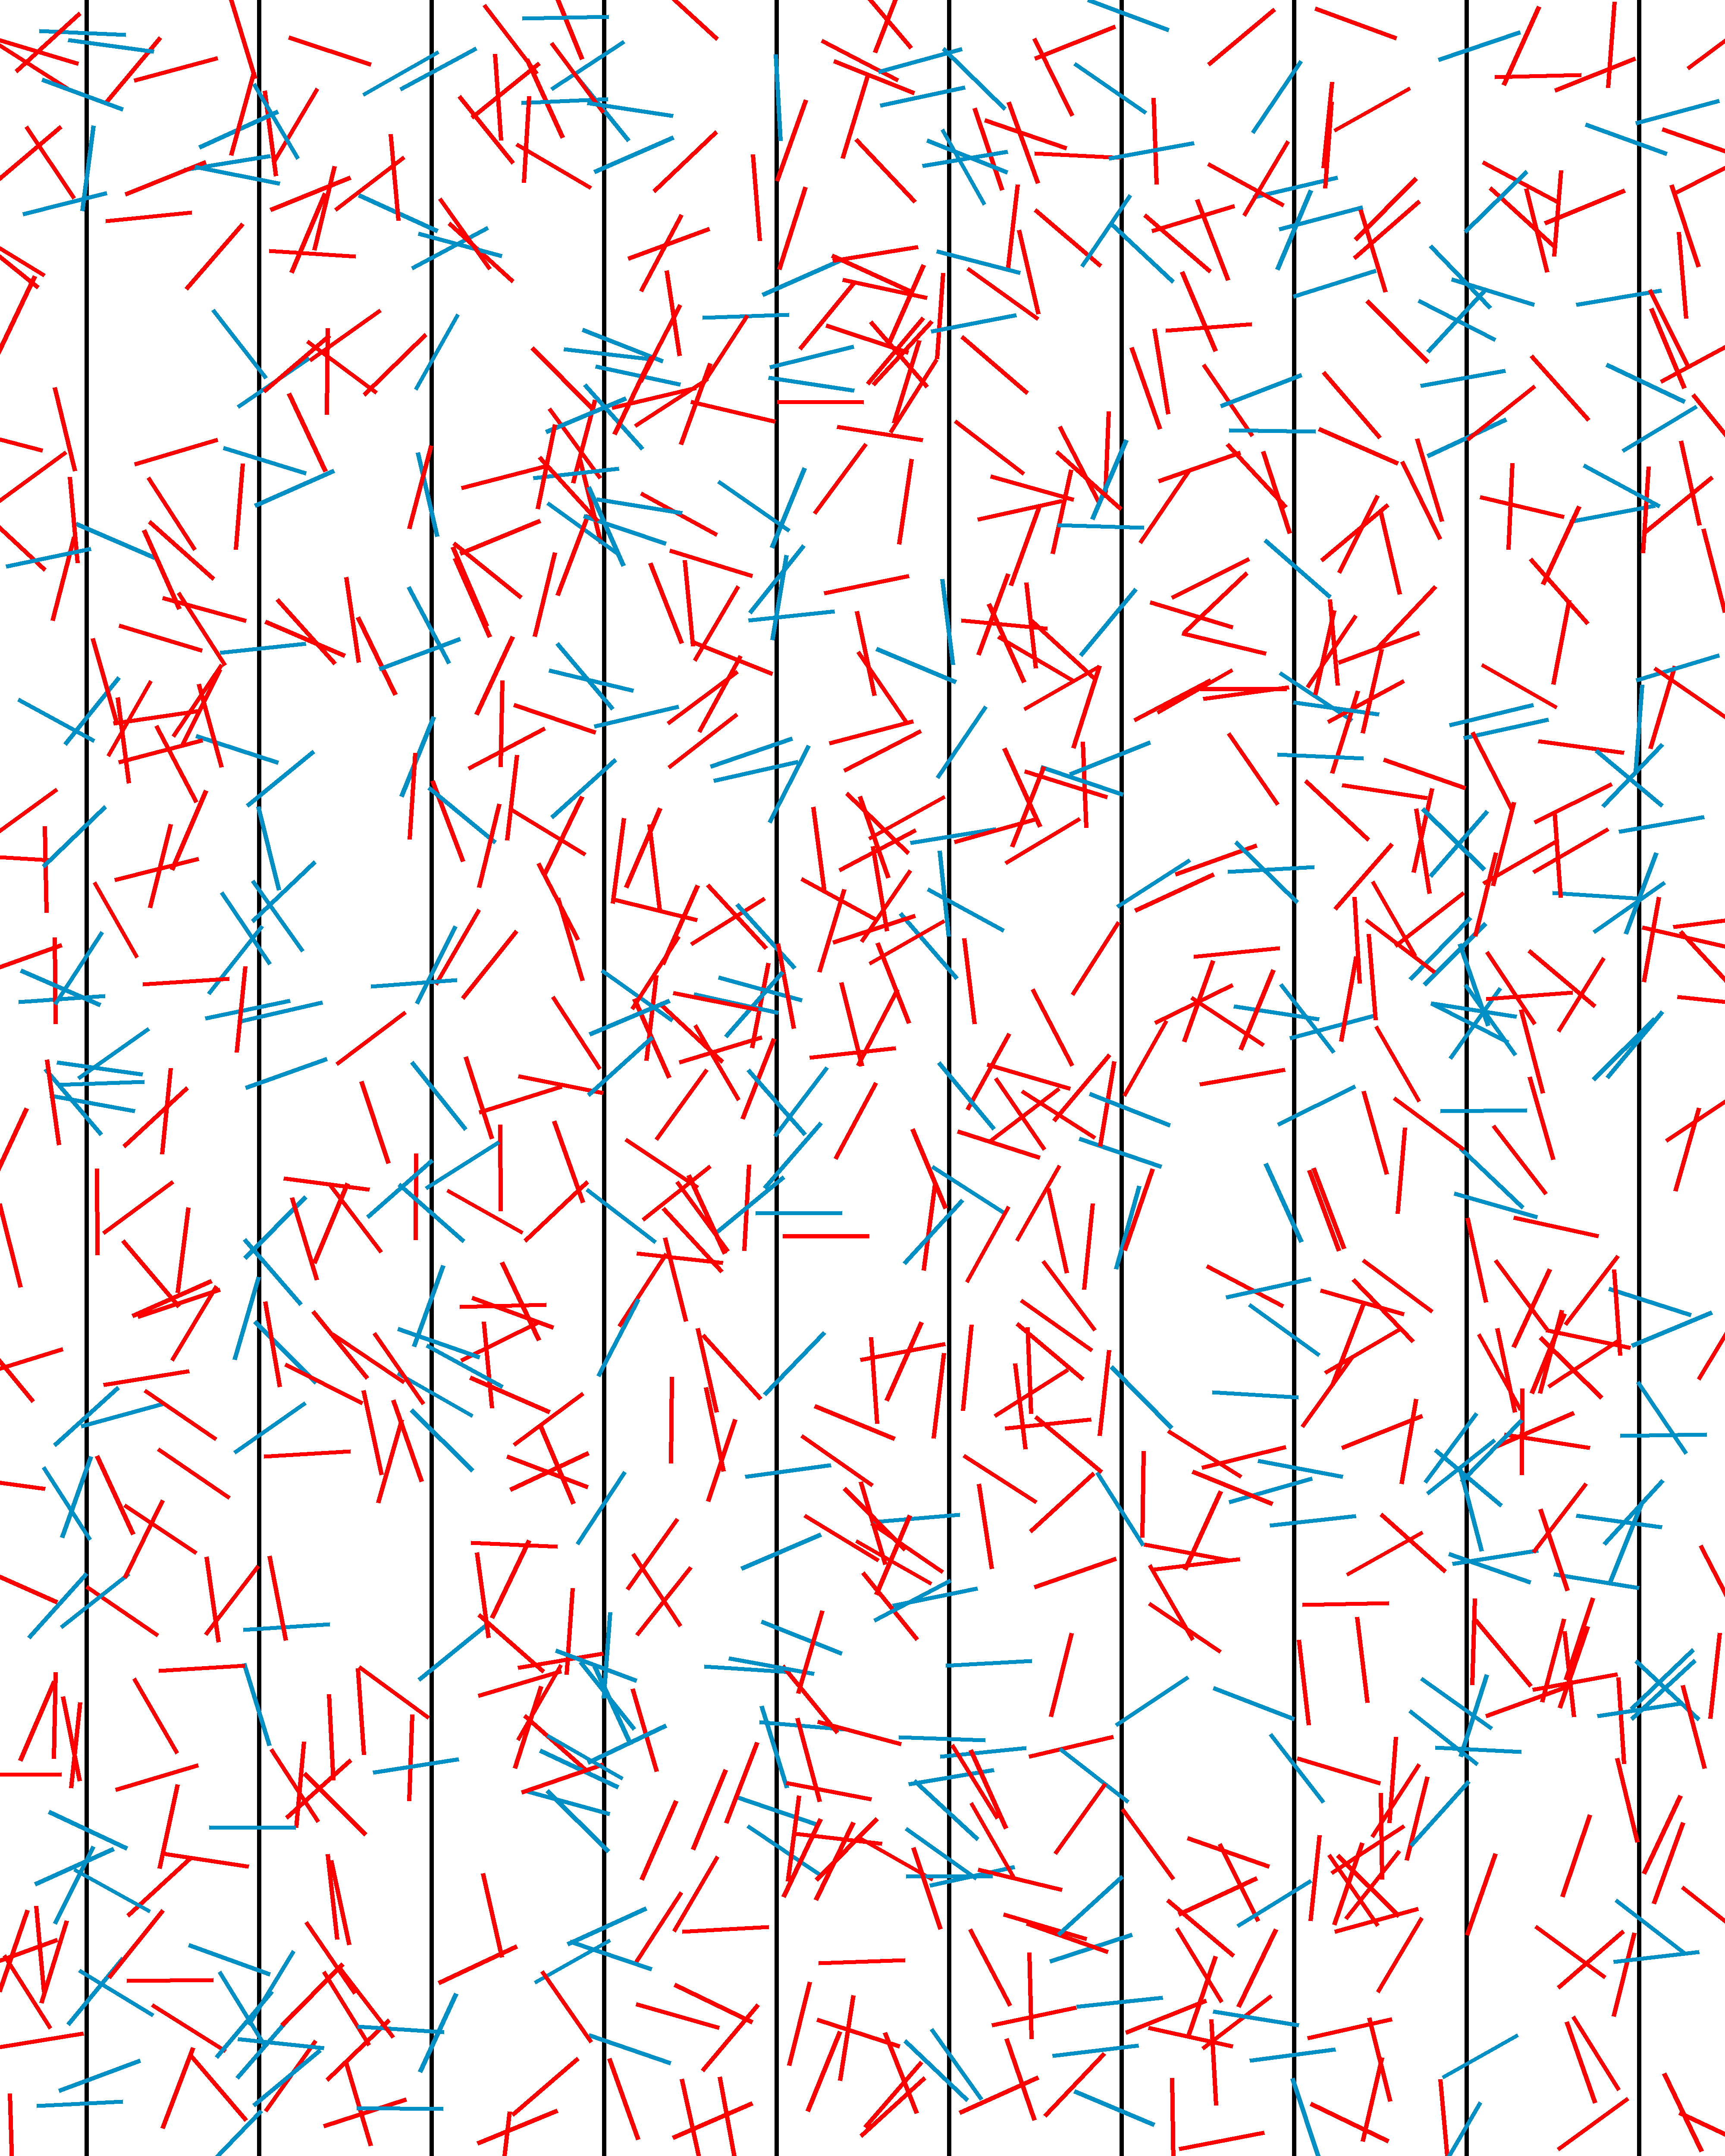
\includegraphics[width=0.45\textwidth]{images/needels.png}
			\caption{Ein Ergebnis der Simulation. Grüne Striche stellen Nadeln dar, die eine Linie schneiden. Rote Striche sind Nadeln, die keine Linie schneiden.}
			\label{fig:needels}
		\end{figure}

		Um zu prüfen, ob eine Nadel eine Linie schneidet, wird der Abstand vom Mittelpunkt der Nadel zur nächsten Linie berechnet. Dann wird mit dem Winkel und der Nadellänge der Abstand in x-Richtung (orthogonal zu den Linien) vom Mittelpunkt der Nadel zur Spitze berechnet. Wenn dieser Abstand größer als der Abstand zur nächsten Linie ist, schneidet die Nadel die Linie:\\
		\texttt{d = (x + line\_dist / 2) \% line\_dist;\\
			dist\_to\_line = min(d, line\_dist - d);\\
			x\_extent = abs(math.cos(angle)) * (needle\_length / 2);\\
			if x\_extent >= dist\_to\_line:}\\
		\\
		Aus dem Ergebnis kann mit der Bibliothek Pillow\cite{Pillow} ein Bild (siehe Abbildung \ref{fig:needels}) erstellt werden, das die geworfenen Nadeln darstellt.

		Für die statistische Auswertung enthält das Programm eine Methode, die eine Reihe von Simulationen durchführt. Für jede Simulation wird dabei die Anzahl der Nadeln, die eine Linie schneiden, in eine JSON-Datei geschrieben. Diese Datei enthält außerdem die Simulationsparameter, sowie die Gesamtanzahl der Nadeln. Dies kann im nächsten Schritt ausgewertet werden. So muss die rechenaufwendige Simulation nicht bei jeder Ausführung der anderen Module des Programms durchgeführt werden.

	\subsection{Die Auswertung}
		Es gibt verschiedene Möglichkeiten die Simulationen mit dem Programm auszuwerten. Als erstes kann man aus der JSON-Datei ein Histogramm erzeugen, das die Häufigkeit eines Ergebnisses darstellt. Erstellt werden die Diagramme mit der Bibliothek matplotlib\cite{matplotlib}. 
		In Abbildung \ref{fig:hist} sieht man, dass die Anzahl an Nadeln, die eine Linie schneiden, annähernd normalverteilt ist.

		\begin{figure}[htb]
			\centering
			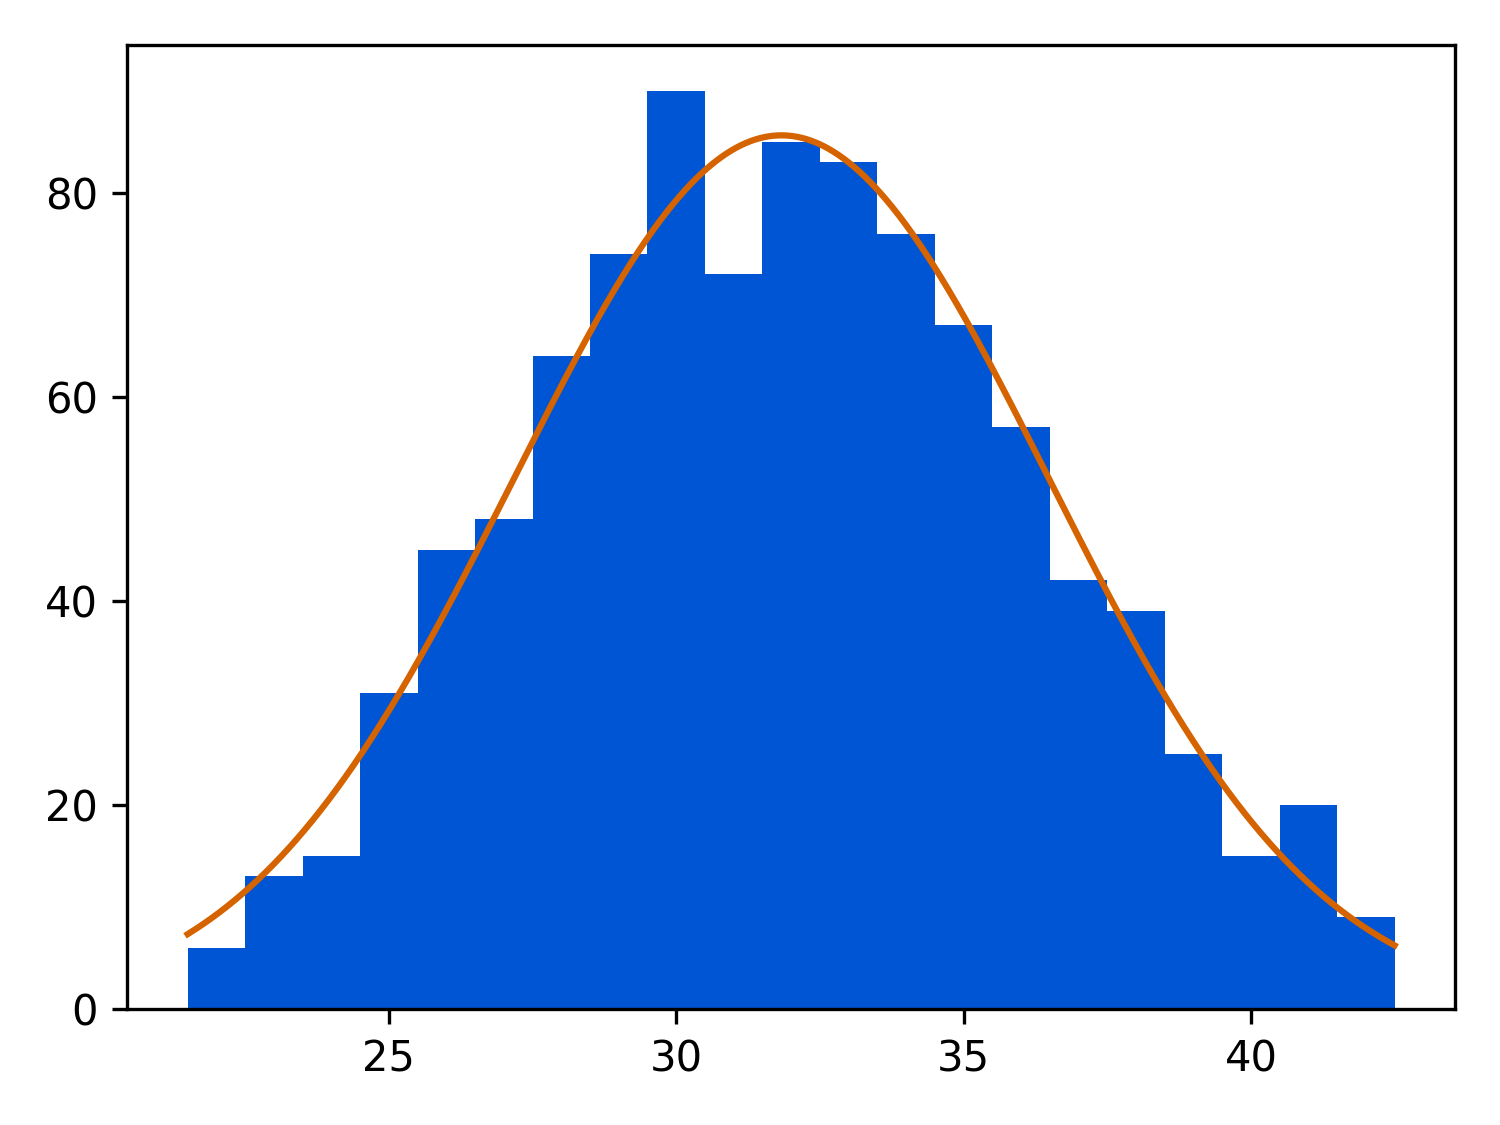
\includegraphics[width=0.45\textwidth]{images/histogram_1000_no_interval_3.png}
			\caption{Histogramm aus 1000 Simulationen mit 100 Nadeln (blau) und Normalverteilung mit gleichen Parametern (orange)}
			\label{fig:hist}
		\end{figure}
		
		Weitere Methoden zur Auswertung werden in den nächsten Kapiteln diskutiert.

\section{Konfidenzintervalle}
		Ein Konfidenzintervall ist ein Bereich, in dem ein bestimmter Parameter mit einer bestimmten Wahrscheinlichkeit liegt. In diesem Kapitel werden Konfidenzintervalle für den Mittelwert $\mu$ und die Varianz $\sigma^2$ untersucht. Diese können verwendet werden um Aussagen über einen unbekannten Parameter der Grundgesamtheit aus den Werten einer Stichprobe zu treffen.

		In Abbildung \ref{fig_mean_interval_hist} ist das $80\%$ Konfidenzintervall des Mittelwerts dargestellt. In diesem Fall ist das Intervall korrekt, da der wahre Mittelwert, der Hochpunkt der orangen Kurve, innerhalb des Intervalls liegt.
		\begin{figure}[h]%
			\centering
			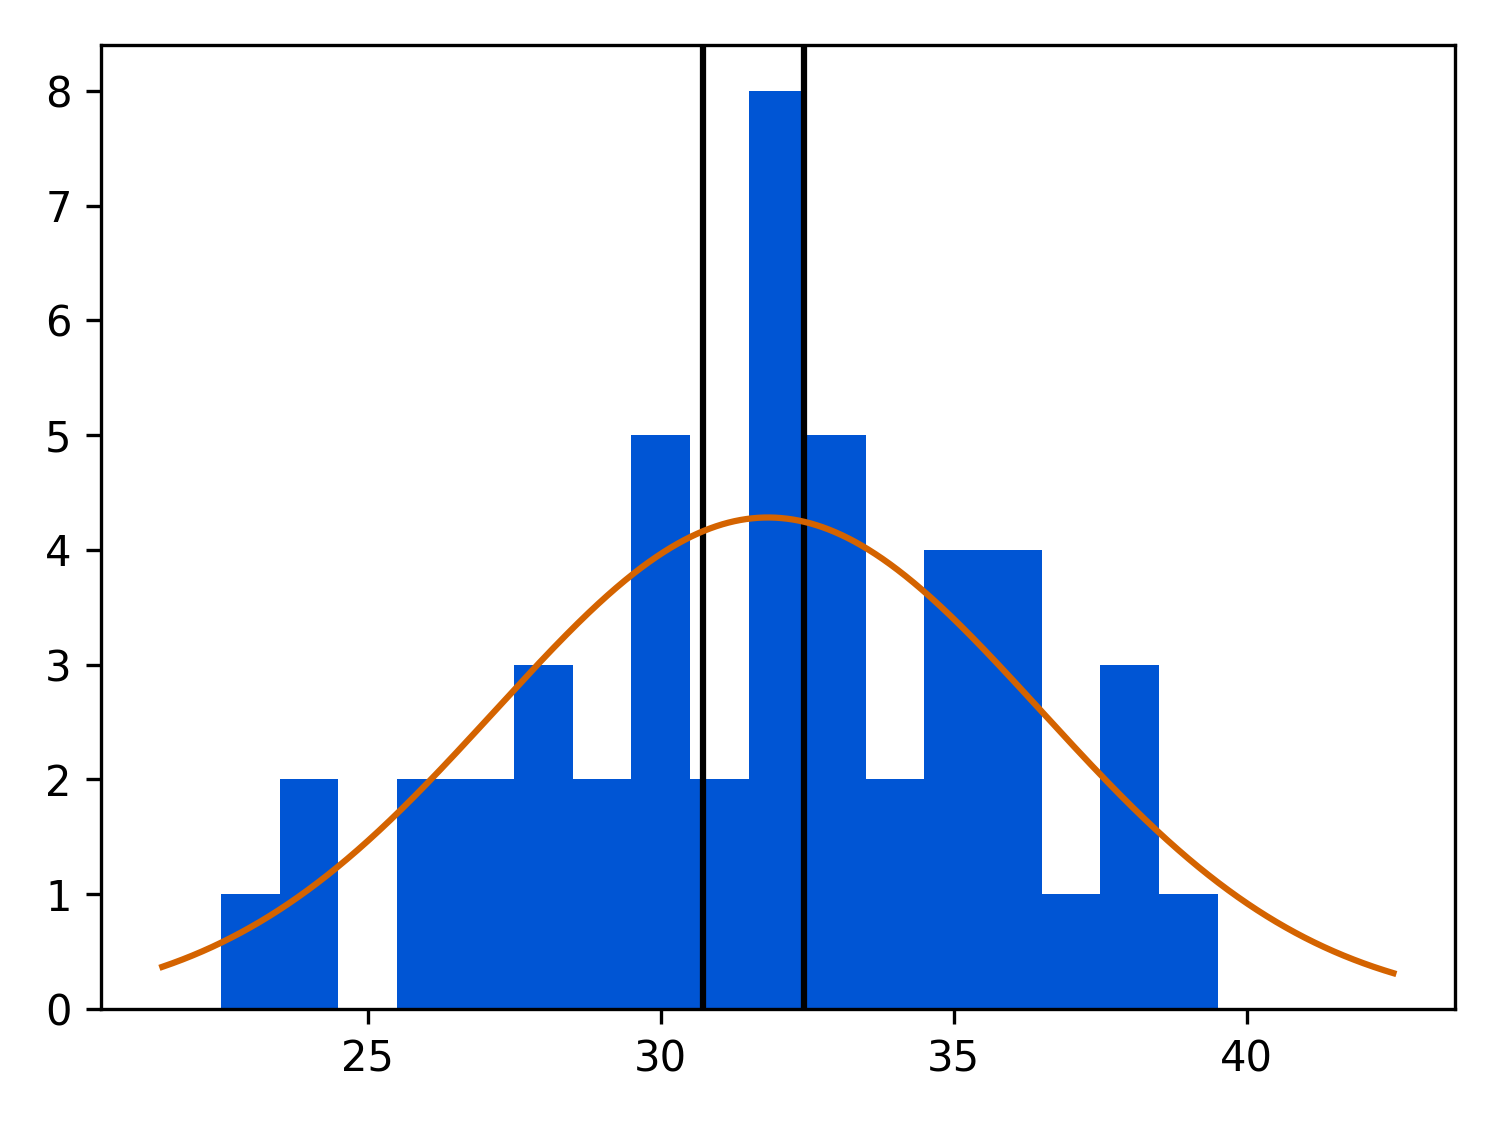
\includegraphics[width=0.9\columnwidth]{images/histogram_50_interval_1.png}
			\caption{Eine Normalverteilung (orange), $50$ nach dieser Verteilung verteilte Werte (blau) und ein aus diesen berechnetes $80\%$ Konfidenzintervall des Mittelwerts (schwarz)}
			\label{fig_mean_interval_hist}
		\end{figure}
	\subsection{Herleitung des Konfidenzintervalls für den Mittelwerts }
		\label{chap_interval_mean_math}
		Gegeben sind $n$ Stichprobenwerte $x_1, x_2, ..., x_n$ und ein Konfidenzniveau $\gamma$ bzw. eine Irrtumswahrscheinlichkeit $\alpha = 1 - \gamma$.
		Ziel ist die Bestimmung von $c_1$ und $c_2$ sodass
		\begin{equation} \label{eq_interval_norm}
		P(c_1 \le \overline{X} \le c_2) = \gamma
		\end{equation}
		gilt.
		Der Durchschnitt der Stichprobe $\overline{x}$ und die geschätzte Standardabweichung $s$ lassen sich direkt aus den Stichprobenwerten berechnen:
		\begin{align}
		\overline{x} &=  \frac{1}{n} \sum_{i=1}^n{x_i} , \\
		s &= \frac{1}{n-1} \sum_{i=1}^n{(x_i - \overline{x})^2} .
		\end{align}
		Um Gleichung \ref{eq_interval_norm} umformen zu können wird eine weitere Zufallsvariable eingeführt:
		\begin{equation} \label{eq_interval_t}
		T = \frac{\overline{X} - \mu}{\frac{S}{\sqrt{n}}} .
		\end{equation}
		Gleichung \ref{eq_interval_norm} kann jetzt mit $T$ umformuliert werden zu:
		\begin{align}
		\gamma &= P(-c \le T \le c) \\ 
		\gamma &= P(T \le c) - P(T \le -c) \nonumber \\
		\gamma &= P(T \le c) - (1 - P(T \le c)) \nonumber \\
		\gamma &= 1 - 2 P(T \le c) \nonumber \\
		\frac{\gamma + 1}{2} &= P(T \le c) .
		\end{align}
		Da $P(T \le c)$ dem Quantil einer t-Verteilung mit $N = n-1$ Freiheitsgraden entspricht, kann der Wert von $c$ aus einer Tabelle abgelesen werden. Ein genaueres Ergebnis bietet die Funktion \texttt{scipy.stats.t.ppf(x, N)} der Python Bibliothek scipy\cite{scipy}.
		Aus der Definition der Zufallsvariable $T$ in Gleichung \ref{eq_interval_t} ergibt sich für die Grenzen des Intervalls:
		\begin{equation}
		c_1 = \overline{x} - \frac{cs}{\sqrt{n}} \mbox{ und } c_2 = \overline{x} + \frac{cs}{\sqrt{n}}.
		\end{equation}

	\subsection{Herleitung des Konfidenzintervalls für die Varianz}
		\label{chap_interval_var_math}
		Die Herleitung des Varianz Intervalls verläuft analog zu der des Konfidenzintervalls des Mittelwerts. Anstelle einer t-Verteilung wird eine Chi-Quadrat-verteilte Zufallsvariable eingeführt:
		\begin{equation} \label{eq_interval_z}
		Z = (n-1)\frac{S^2}{\sigma^2} .
		\end{equation}
		\begin{align}
		\gamma &= P(c_1 \le Z \le c_2) \\
		\gamma &= P(Z \le c_2) - P(Z \le c_1) \nonumber \\
		P(Z \le c_1) &= \frac{1}{2} (1-\gamma) \\
		P(Z \le c_2) &= \frac{1}{2} (1+\gamma)
		\end{align}
		Hier entspricht $P(T \le c_i)$ jeweils einem Quantil einer Chi-Quadrat-Verteilung mit $N = n-1$ Freiheitsgraden, dies kann mit \texttt{scipy.stats.chi2.ppf(x, N)}\cite{scipy} berechnet werden.
		Aus der Definition der Zufallsvariable $Z$ in Gleichung \ref{eq_interval_z} ergibt sich das Konfidenzintervall der Varianz:
		\begin{equation}
		(n-1)  \frac{s^2}{c_2} \le \sigma^2 \le (n-1)  \frac{s^2}{c_1}.
		\end{equation}

	\subsection{Empirischer Beweis}
		\label{chap_interval_prove}
		Insbesondere durch die Annahmen, die in Gleichung \ref{eq_interval_t} und \ref{eq_interval_z} eingeführten  Zufallsvariablen $T$ und $Z$, würden genau einer t-Verteilung bzw. Chi-Quadrat-Verteilung mit jeweils $N = n-1$ Freiheitsgraden entsprechen, ist die Herleitung alleine nur bedingt geeignet um die daraus gewonnen Formeln zu plausibilisieren.

		Um die Korrektheit der in Abschnitt \ref{chap_interval_mean_math} hergeleiteten Formeln zu bestätigen wurde ein empirischer Beweis durchgeführt. Die Berechnung der Konfidenzintervalle wurde in Python implementiert, so können diese beliebig oft mit den von der Simulation erstellten Daten aus Abschnitt \ref{chap_sim_results} durchgeführt werden.

		Der folgende Test wird separat für mehrere Werte von $\gamma \in [0, 1]$ durchgeführt. Es wird für $n = 20$ Werte das Konfidenzintervall des Mittelwerts und der Varianz mit einem Konfidenzniveau $\gamma$ gebildet. Durch den in Kapitel \ref{chap_buffon_needle} hergeleiteten Wert für $p$ kann der theoretisch zu erwartende Mittelwert und die Varianz berechnet werden:
		\begin{align}
		E(X) &= n \cdot p , \\
		\sigma &= n \cdot p (1-p) , \nonumber \\
		Var(X) &= \sigma^2 = (n \cdot p (1-p))^2 .
		\end{align}

		Es wird überprüft, ob der Erwartungswert und die Varianz der Grundgesamtheit innerhalb oder außerhalb des geschätzten Intervalls liegen.

		Dieser Vorgang wird in $10^5$ Durchläufen wiederholt und dabei der Anteil an korrekten Intervallen gezählt. Daraus wird das Verhältnis zwischen dem tatsächlichen Anteil an korrekten Intervallen und $\gamma$ berechnet. Wenn die Formeln stimmen ist der Erwartungswert dieses Verhältnisses $1$.

		Um zu zeigen, dass diese Methode der Überprüfung funktioniert, wurden nicht nur die hergeleiteten Formeln, sondern auch absichtlich falschen Formeln überprüft. Für die falschen Formeln wurden $N = n$ Freiheitsgrade angenommen (richtig sind $N = n-1$). Abhängig von den Parametern ist dieser Fehler schwer zu erkennen, da die Ergebnisse sehr nahe an den eigentlich richtigen liegen.

		Die Ergebnisse sind in Abbildung \ref{fig_mean_interval_dot} und \ref{fig_var_interval_dot} dargestellt. Dabei ist klar zu erkennen, dass die mit den richtigen Formeln berechneten Ergebnisse nahe an $1$ liegen und die mit den falschen Formeln berechneten Ergebnisse deutlich von $1$ abweichen. Dies bestätigt die Korrektheit der Formeln und des Testverfahrens.

		\begin{figure}[h]%
			\centering
			\begin{subfigure}[c]{1\columnwidth}
				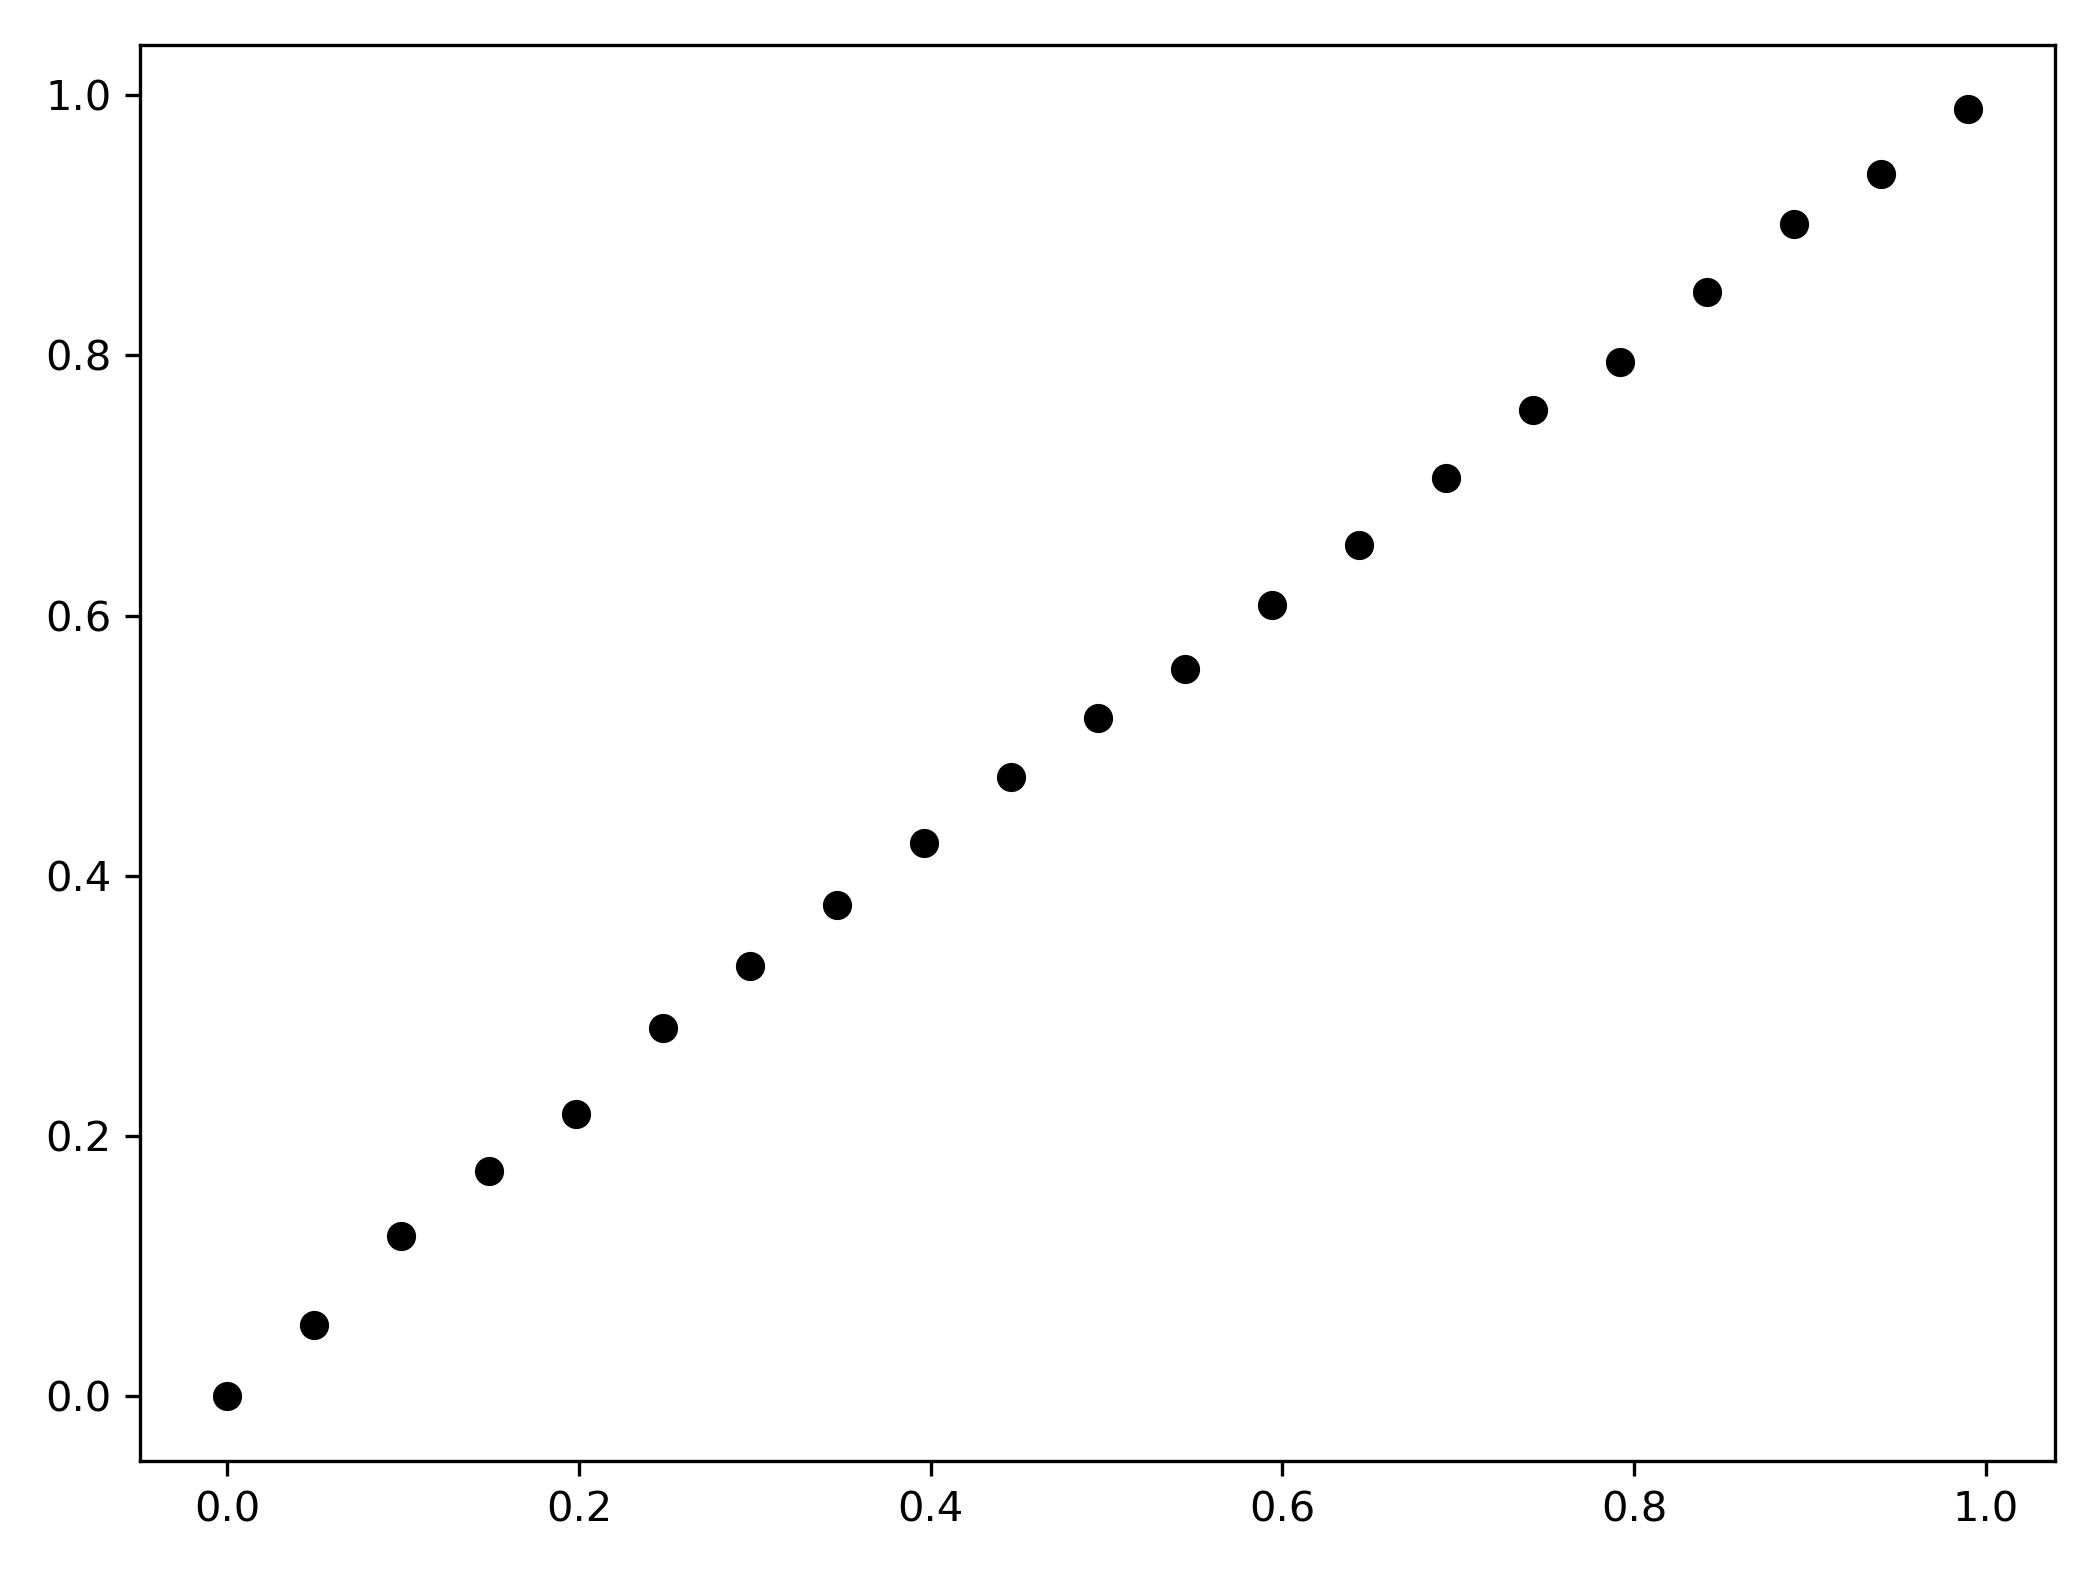
\includegraphics[width=0.9\columnwidth]{images/mean_interval.png}
				\caption{Konfidenzintervall des Mittelwerts}
				\label{fig_mean_interval_dot}
			\end{subfigure}
			\begin{subfigure}[c]{1\columnwidth}
				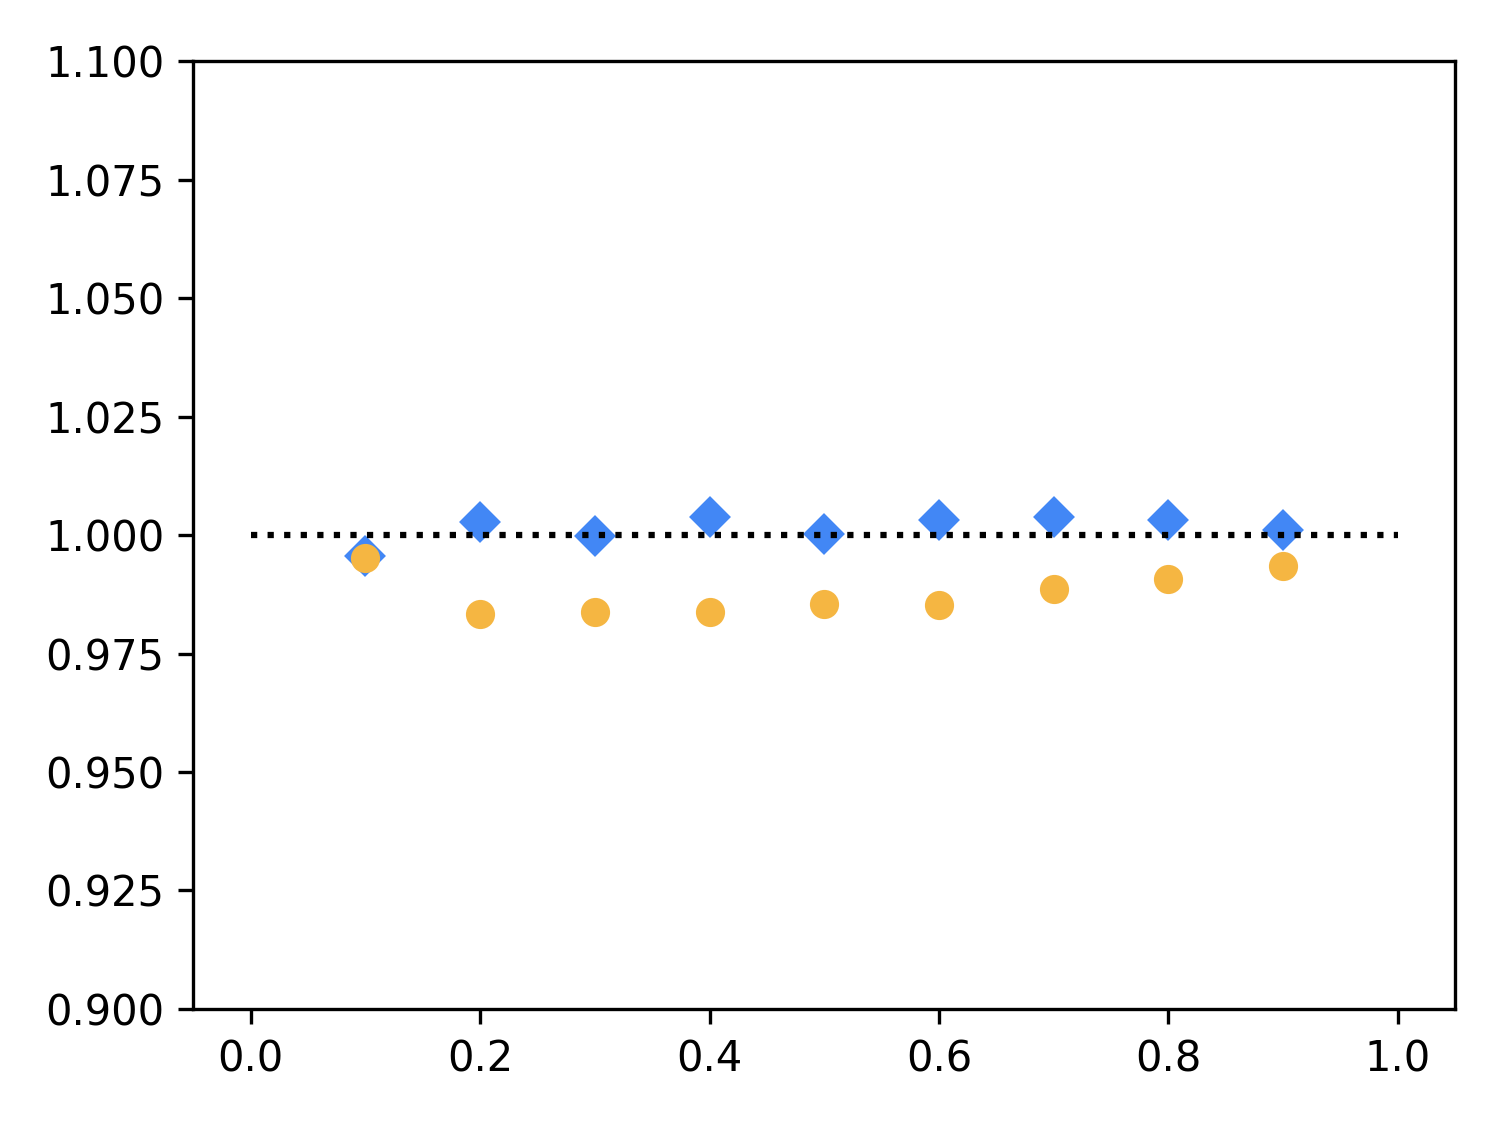
\includegraphics[width=0.9\columnwidth]{images/var_interval.png}
				\caption{Konfidenzintervall der Varianz}
				\label{fig_var_interval_dot}
			\end{subfigure}
			\caption{Abweichung des tatsächlichen Anteils an korrekt geschätzten Intervallen von dem Konfidenzniveau (y-Achse) für verschiedene Konfidenzniveaus (x-Achse) von dem idealen Wert (schwarz) für Ergebnisse der richtigen Formeln (blau) und der falschen Formeln (gelb).}
		\end{figure}


\section{Parametertests}
		Mit einem Parametertest kann eine Aussage darüber getroffen werden, ob ein bestimmter Wert eines Parameters angesichts der bekannten Werte einer Stichprobe plausibel ist. In diesem Kapitel wird der Parametertest für den Mittelwert $\mu$ untersucht. Dieser kann beispielsweise verwendet werden, um Angaben eines Herstellers zu überprüfen.
	\subsection{Herleitung des Parametertests für den Mittelwert}
		Gegeben sind $n$ Stichprobenwerte $x_1, x_2, ..., x_n$ und ein Konfidenzniveau $\gamma$ bzw. eine Irrtumswahrscheinlichkeit $\alpha = 1 - \gamma$. Es soll getestet werden, ob ein angegebener Wert des Mittelwerts der Grundgesamtheit $\mu_0$ korrekt ist.

		Das Ziel ist die Entscheidung zwischen einer Nullhypothese $H_0$ ($\mu = \mu_0$) und einer Alternativhypothese $H_1$ ($\mu \ne \mu_0$).

		Das Vorgehen ähnelt dem Schätzen eines Konfidenzintervalls für den Mittelwert. Es wird die Zufallsvariable $T$ eingeführt (Gleichung \ref{eq_interval_t}), mit dieser kann der Test formuliert werden als:
		\begin{equation}
		P(-c \le T \le c) = \gamma .
		\end{equation}
		$c$ wird wieder aus den Quantilen der t-Verteilung berechnet. Es wird aber $c$ nicht aus $T$ in $X$ rücktransformiert um die Grenzen des Konfidenzintervalls zu erhalten, sondern der Mittelwert der Stichprobe wird nach $T$ transformiert mit:
		\begin{equation}
		\hat{t} = \frac{\overline{x} - \mu_0}{\frac{s}{\sqrt{n}}} .
		\end{equation}

		Dann ist $H_0$ mit einer Wahrscheinlichkeit $\gamma$ wahr, wenn
		\begin{equation}
		-c \le \hat{t} \le c
		\end{equation}
		gilt. Andernfalls ist $H_1$ wahr.

		Mit einer höheren Irrtumswahrscheinlichkeit $\alpha = 1 - \gamma$ sinkt die Wahrscheinlichkeit $H_0$ fälschlich abzulehnen, dafür steigt die Wahrscheinlichkeit $H_0$ fälschlich anzunehmen.
	\subsection{Empirischer Beweis}
		Dass die hergeleiteten Formeln gelten, ist auch hier durch die Einführung einer weiteren Zufallsvariable nicht sofort plausibel.

		Das Vorgehen entspricht im Wesentlichen dem aus Abschnitt \ref{chap_interval_prove}. Die Auswertung gestaltet sich etwas einfacher, da der Parametertest direkt einen Wahrheitswert liefert, die Annahme oder Ablehnung von $H_0$.

		Die Ergebnisse sind in Abbildung \ref{fig_test_mean_dot} zu sehen. Das Verhältnis aus negativen Parametertests und der Irrtumswahrscheinlichkeit bei der richtigen Formeln liegen wieder nahe an $1$ und das der falschen Formeln weichen deutlich von $1$ ab. Dies bestätigt die Korrektheit der Formeln und des Testverfahrens.

		\begin{figure}[H]
			\centering
			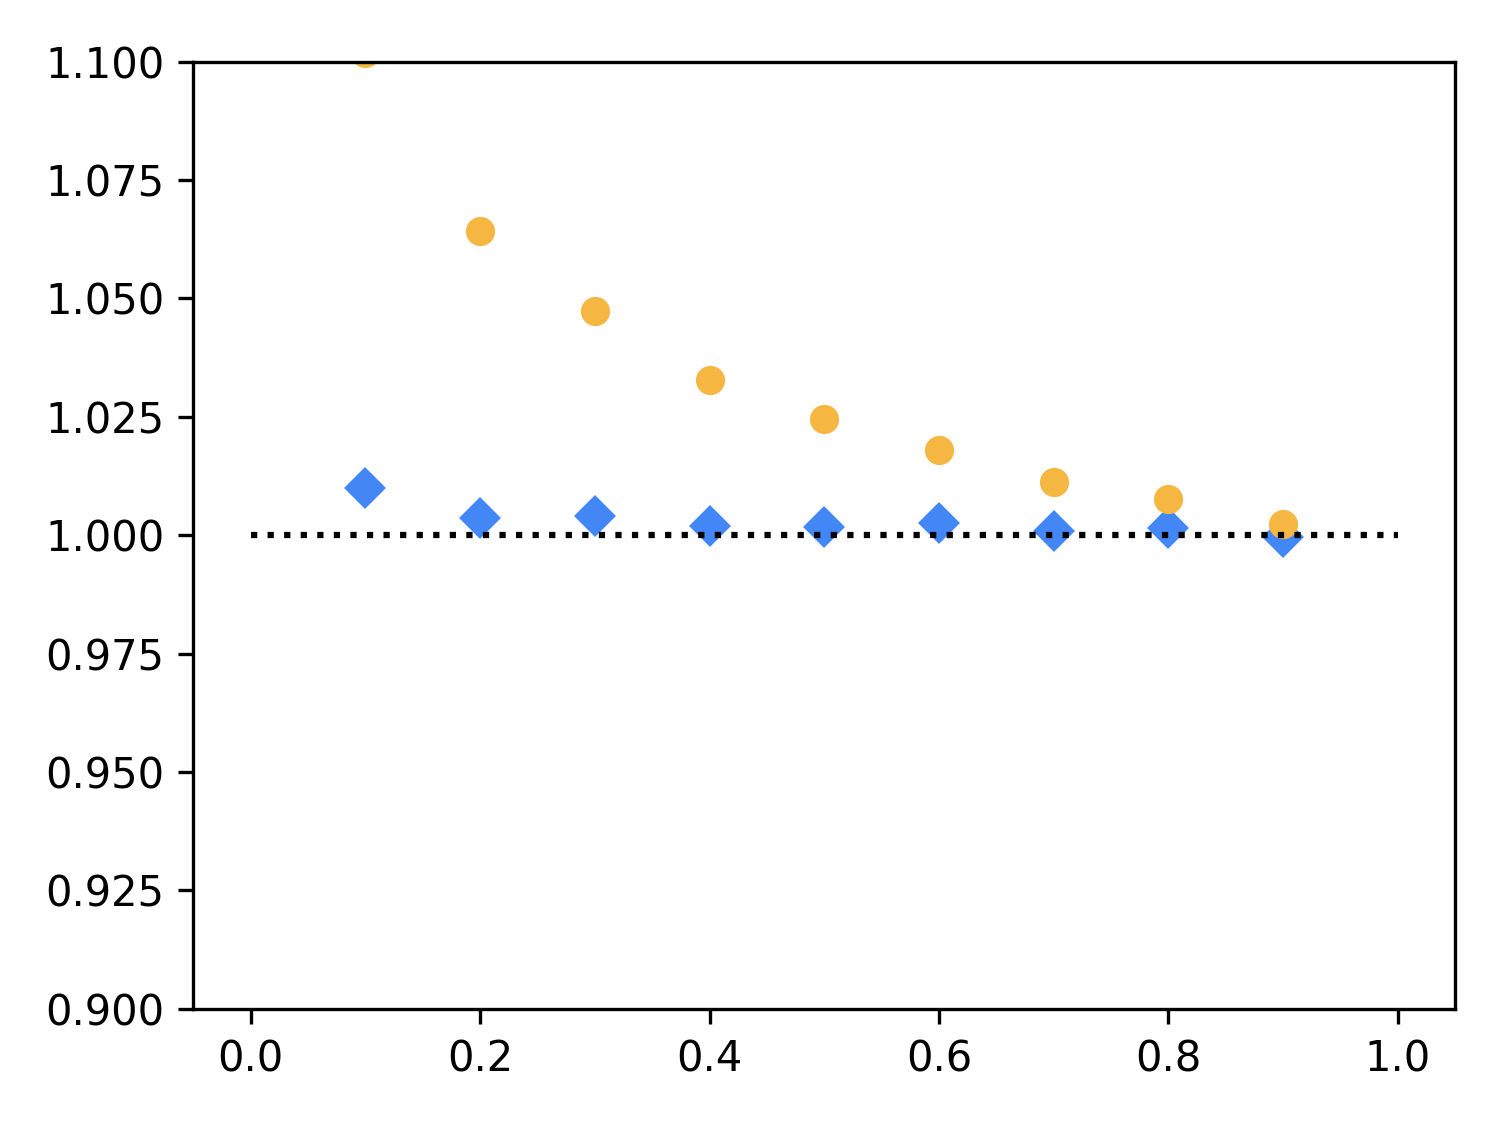
\includegraphics[width=0.9\columnwidth]{images/mean_test.png}
			\caption{Abweichung des Anteils negativer Parametertests von der Irrtumswahrscheinlichkeit (y-Achse) für verschiedene Irrtumswahrscheinlichkeiten (x-Achse) von dem idealen Wert (schwarz) für Ergebnisse der richtigen Formeln (blau) und der falschen Formeln (gelb).}
			\label{fig_test_mean_dot}
		\end{figure}

\section{Experimenteller Test von Lazzarini}
	Es gab mehrere Versuche durch eine praktische Durchführung des Buffonschen Nadelexperiments den Wert für $\pi$ anzunähern. Mario Lazzarini soll 1901 das zur Zeit umfangreichste Experiment durchgeführt haben. Hierfür baute er eigens eine Maschine und führte das Experiment mit 3408 Nadelwürfen durch. Das Längenverhältnis betrug hierbei ${\tfrac {l}{d}={\tfrac {5}{6}}}$. Mit einem Ergebnis von 1808 Nadeln, die eine Linie schneiden, schaffte Lazzarini es mit diesem Experiment den Wert von $\pi$ auf sechs Nachkommastellen anzunähern. Diese hohe Genauigkeit wurde von vielen als Glückstreffer oder Fälschung gesehen.\cite{Badger}

	Wie glaubwürdig Lazzarinis Ergebnis war, lässt sich mithilfe eines Konfidenzintervalls bestimmen.
	In Lazzarinis Versuch beträgt die geschätzte Standardabweichung $s = 0.249141$.
	Für ein Konfidenzniveau von $\gamma = 0.95$ ergibt sich
	\begin{equation}
	P(T \le c) = \frac{\gamma + 1}{2} = \frac{0.95 + 1}{2} = 0.975 .
	\end{equation}
	Mit $N = n - 1 = 3407$ Freiheitsgraden erhält man aus der t-Verteilung $c = 1,96066$.
	Somit erreichte Lazzarini bei seinem Experiment zu $95\%$ eine Genauigkeit von
	\begin{align}
	\Delta \mu &= \frac{cs}{\sqrt{n}} \\
	&= \frac{1,96066 \cdot 0.249141}{\sqrt{3408}} \nonumber \\
	&= 8,367538 \cdot 10 ^{-3} \nonumber
	\end{align}
	oder schlechter für den Mittelwert. Der Zusammenhang von $\pi$ und dem Mittelwert, der hier der Wahrscheinlichkeit $P$ entspricht, da es sich um eine Binomialverteilung handelt, ist durch folgende Formel gegeben (siehe Kapitel \ref{chap_buffon_needle}):
	\begin{equation}
	P(x) = \frac{2l}{\pi d}.
	\end{equation}
	So erhält man als erwartete Genauigkeit für den ermittelten Wert von $\pi$
	\begin{align}
	\Delta \pi &= \pi - \frac{2 \cdot \frac{l}{d}}{P + \Delta \mu} \\
	&= \pi - \frac{2 \cdot \frac{5}{6}}{\frac{1808}{3408} + 8,367538 \cdot 10 ^{-3}} \nonumber \\
	&= 0.048781 \nonumber .
	\end{align}
	Das ist deutlich ungenauer als $\Delta \pi = 0,5 * 10^{-6}$, was sechs Nachkommastellen entsprechen würde.
	Die Genauigkeit von dem ermittelten Wert für $\pi$ von Lazzarini von 6 Nachkommastellen war also nicht zu erwarten.
	
	Dabei könnte es sich um bloßen Zufall handeln. Die merkwürdige Anzahl an Nadelwürfen ($3408$) ist aber besonders verdächtig. Sein Ergebnis entspricht exakt der auch zu diesem Zeitpunkt bekannten Approximation $\pi \approx \frac{355}{113}$.
	Um diese Approximation mit dem von ihm verwendeten Verhältnis ${\tfrac {l}{d}={\tfrac {5}{6}}}$ zu erhalten, muss das Verhältnis von Nadeln, die eine Linie schneiden, zu allen Nadeln exakt
	\begin{equation}
	\frac{5}{3} \frac{1}{\pi}  \approx \frac{5}{3} \cdot \frac{113}{355} = \frac{113}{213}
	\end{equation}
	sein.
	Seine Anzahl an Würfen ist genau ein ganzes Vielfaches des Nenners:
	\begin{equation}
	16 \cdot 213 = 3408
	\end{equation}
	Dies spricht stark dafür, dass Lazzarini die Parameter des Experiments mit dem direkten Ziel eine schon bekannte Approximation zu treffen ausgelegt hat oder die Daten sogar frei erfunden hat. \cite{Badger}
	
	
\section{Ergebnisse und Diskussion}
	In dieser Arbeit wurden Konfidenzintervalle und  Parametertests als hilfreiche Werkzeuge bei der Analyse von statistischen Daten eingeführt. Dabei wurden die dafür notwendigen Formeln hergeleitet und durch einen empirischen Beweis plausibilisiert.
	Auch die Korrektheit des dabei verwendeten Testverfahrens wurde durch das Testen absichtlich falschen Formeln auf die Probe gestellt. Dabei hat das Testverfahren die falschen Formeln als solche identifizieren können und die Korrektheit der richtigen Formeln bestätigt.
	
	Das Buffonsche Nadelproblem wurde erläutert und die dabei relevanten Formeln hergeleitet. Außerdem wurde das Experiment in einer Simulation durchgeführt.
	Zum Abschluss wurde ein spezieller Fall, die Durchführung des Experiments von Lazzarini, genauer untersucht. Dabei wurden durch ein Konfidenzintervall und Hintergrundinformationen gezeigt, dass Lazzarini vermutlich absichtlich manipuliert hat, um ein gutes Ergebnis aus dem Experiment zu erhalten.
	
	\bigskip
	\noindent
	Der Quellcode des erstellten Programms und dieser Arbeit ist öffentlich zugänglich unter:\\ \url{https://github.com/DavidRisch/buffon}.

\newpage
\begin{thebibliography}{99}
	\bibitem{MathWorld}Weisstein, Eric W.: {\textit Buffon's Needle Problem.}, From MathWorld--A Wolfram Web Resource. \url{https://mathworld.wolfram.com/BuffonsNeedleProblem.html}
	\bibitem{Pillow}Pillow: \url{https://pillow.readthedocs.io/en/stable/}
	\bibitem{matplotlib}matplotlib: \url{https://matplotlib.org/}
	\bibitem{scipy}scipy: \url{https://www.scipy.org/}
	\bibitem{Badger}Lee Badger: Lazzarini’s Lucky Approximation of $\pi$, Mathematics Magazine, Band 67, 1994, 83-85
\end{thebibliography}

\end{document}